%%
%% This is file `sample-sigconf-biblatex.tex',
%% generated with the docstrip utility.
%%
%% The original source files were:
%%
%% samples.dtx  (with options: `all,proceedings,sigconf-biblatex')
%% 
%% IMPORTANT NOTICE:
%% 
%% For the copyright see the source file.
%% 
%% Any modified versions of this file must be renamed
%% with new filenames distinct from sample-sigconf-biblatex.tex.
%% 
%% For distribution of the original source see the terms
%% for copying and modification in the file samples.dtx.
%% 
%% This generated file may be distributed as long as the
%% original source files, as listed above, are part of the
%% same distribution. (The sources need not necessarily be
%% in the same archive or directory.)
%%
%%
%% Commands for TeXCount
%TC:macro \cite [option:text,text]
%TC:macro \citep [option:text,text]
%TC:macro \citet [option:text,text]
%TC:envir table 0 1
%TC:envir table* 0 1
%TC:envir tabular [ignore] word
%TC:envir displaymath 0 word
%TC:envir math 0 word
%TC:envir comment 0 0
%%
%% The first command in your LaTeX source must be the \documentclass
%% command.
%%
%% For submission and review of your manuscript please change the
%% command to \documentclass[manuscript, screen, review]{acmart}.
%%
%% When submitting camera ready or to TAPS, please change the command
%% to \documentclass[sigconf]{acmart} or whichever template is required
%% for your publication.
%%
%%

\documentclass[sigconf,natbib=true]{acmart}
\usepackage{tikz}
\usepackage{pgf-pie}
%%
%% \BibTeX command to typeset BibTeX logo in the docs
\AtBeginDocument{%
  \providecommand\BibTeX{{%
    Bib\TeX}}}

%% Rights management information.  This information is sent to you
%% when you complete the rights form. These commands have SAMPLE
%% values in them; it is your responsibility as an author to replace
%% the commands and values with those provided to you when you
%% complete the rights form.
\setcopyright{acmlicensed}
\copyrightyear{2018}
\acmYear{2018}
% \acmDOI{XXXXXXX.XXXXXXX}
%% These commands are for a PROCEEDINGS abstract or paper.
% \acmConference[Conference acronym 'XX]{Make sure to enter the correct
%   conference title from your rights confirmation email}{June 03--05,
%   2018}{Woodstock, NY}
%%
%%  Uncomment \acmBooktitle if the title of the proceedings is different
%%  from ``Proceedings of ...''!
%%
%%\acmBooktitle{Woodstock '18: ACM Symposium on Neural Gaze Detection,
%%  June 03--05, 2018, Woodstock, NY}
% \acmISBN{978-1-4503-XXXX-X/2018/06}


%%
%% Submission ID.
%% Use this when submitting an article to a sponsored event. You'll
%% receive a unique submission ID from the organizers
%% of the event, and this ID should be used as the parameter to this command.
%%\acmSubmissionID{123-A56-BU3}

%%
%% For managing citations, it is recommended to use bibliography
%% files in BibTeX format.
%%
%% You can then either use BibTeX with the ACM-Reference-Format style,
%% or BibLaTeX with the acmnumeric or acmauthoryear sytles, that include
%% support for advanced citation of software artefact from the
%% biblatex-software package, also separately available on CTAN.
%%
%% Look at the sample-*-biblatex.tex files for templates showcasing
%% the biblatex styles.
%%


%%
%% The majority of ACM publications use numbered citations and
%% references, obtained by selecting the acmnumeric BibLaTeX style.
%% The acmauthoryear BibLaTeX style switches to the "author year" style.
%%
%% If you are preparing content for an event
%% sponsored by ACM SIGGRAPH, you must use the acmauthoryear style of
%% citations and references.
%%
%% Bibliography style
% \RequirePackage[
%   datamodel=acmdatamodel,
%   style=acmnumeric,
%   backend=biber,
%   ]{biblatex}
\bibliographystyle{ACM-Reference-Format}

%%
%% end of the preamble, start of the body of the document source.
\begin{document}

%%
%% The "title" command has an optional parameter,
%% allowing the author to define a "short title" to be used in page headers.
\title{The Name of the Title Is Hope}

%%
%% The "author" command and its associated commands are used to define
%% the authors and their affiliations.
%% Of note is the shared affiliation of the first two authors, and the
%% "authornote" and "authornotemark" commands
%% used to denote shared contribution to the research.

\author{Kiane Heather S. Bedonia}
\email{ksbedonia@up.edu.ph}
\affiliation{%
  \institution{Institute of Computer Science}
  \city{University of the Philippines}
  \state{Los Baños, Laguna}
  \country{Philippines}
}

\author{Yosef Christian M. Cuenca}
\email{ymcuenca@up.edu.ph}
\affiliation{%
  \institution{Institute of Computer Science}
  \city{University of the Philippines}
  \state{Los Baños, Laguna}
  \country{Philippines}
}

\author{Alyanna P. Galido}
\email{apgalido@up.edu.ph}
\affiliation{%
  \institution{Institute of Computer Science}
  \city{University of the Philippines}
  \state{Los Baños, Laguna}
  \country{Philippines}
}

\author{Kurt Princip Gavryl T. Sumallo}
\email{ksbedonia@up.edu.ph}
\affiliation{%
  \institution{Institute of Computer Science}
  \city{University of the Philippines}
  \state{Los Baños, Laguna}
  \country{Philippines}
}

%%
%% By default, the full list of authors will be used in the page
%% headers. Often, this list is too long, and will overlap
%% other information printed in the page headers. This command allows
%% the author to define a more concise list
%% of authors' names for this purpose.
\renewcommand{\shortauthors}{Bedonia et al.}

%%
%% The abstract is a short summary of the work to be presented in the
%% article.
\begin{abstract}
  A clear and well-documented \LaTeX\ document is presented as an
  article formatted for publication by ACM in a conference proceedings
  or journal publication. Based on the ``acmart'' document class, this
  article presents and explains many of the common variations, as well
  as many of the formatting elements an author may use in the
  preparation of the documentation of their work.
\end{abstract}

%%
%% The code below is generated by the tool at http://dl.acm.org/ccs.cfm.
%% Please copy and paste the code instead of the example below.
%%
\begin{CCSXML}
<ccs2012>
   <concept>
       <concept_id>10003120.10003121.10011748</concept_id>
       <concept_desc>Human-centered computing~Empirical studies in HCI</concept_desc>
       <concept_significance>500</concept_significance>
       </concept>
   <concept>
       <concept_id>10010405.10010489.10010490</concept_id>
       <concept_desc>Applied computing~Computer-assisted instruction</concept_desc>
       <concept_significance>500</concept_significance>
       </concept>
    <concept>
       <concept_id>10010405.10010489.10010493</concept_id>
       <concept_desc>Applied computing~Learning management systems</concept_desc>
       <concept_significance>300</concept_significance>
       </concept>
 </ccs2012>
\end{CCSXML}

\ccsdesc[500]{Human-centered computing~Empirical studies in HCI}
\ccsdesc[300]{Applied computing~Learning management systems}
\ccsdesc[500]{Applied computing~Computer-assisted instruction}

\ccsdesc[500]{Human-centered computing~Empirical studies in HCI}

%%
%% Keywords. The author(s) should pick words that accurately describe
%% the work being presented. Separate the keywords with commas.
\keywords{AI in the Classroom, Generative AI, Large Language Models, AI Chatbot}
%% A "teaser" image appears between the author and affiliation
%% information and the body of the document, and typically spans the
%% page.
\begin{teaserfigure}
  \includegraphics[width=\textwidth]{stella_hero.png}
  \caption{Hero of the STELLA Landing Page.}
  \Description{
    The STELLA hero banner on a green background featuring the platform's full name: System for Transparent Engagement with LLMs for Learning and Assessment. The design includes a curved dotted path with a star icon. The image displays three sections highlighting platform benefits: integration with multiple language models (showing icons for various AI platforms), compatibility with existing educational platforms (showing LMS integration icons), and support from academic institutions (showing university logos). The overall design conveys an educational technology solution for transparent AI use in academic settings.}
\end{teaserfigure}

\received{21 May 2025}
% \received[revised]{12 March 2009}
% \received[accepted]{5 June 2009}

%%
%% This command processes the author and affiliation and title
%% information and builds the first part of the formatted document.
\maketitle

\section{Introduction}
In the rapidly evolving landscape of education shaped by artificial intelligence (AI), educational institutions are faced with the urgent need to adapt teaching and learning practices that not only incorporate emerging technologies but also preserve essential academic values. The proliferation of large language models (LLMs) presents both opportunities and challenges—while they can support student learning through personalized assistance and streamlined feedback, their misuse or unchecked integration can risk undermining critical thinking, creativity, and academic integrity. Recognizing this duality, the development of STELLA (System for Transparent Engagement with LLMs for Learning and Assessment) was conceived to bridge this gap and foster a transparent, ethical, and effective environment for AI-assisted coursework.

\subsection{Background and Rationale}
It is undeniable that the increased access to and capabilities of generative AI (GenAI) and large language models (LLMs) have radically transformed how students and teachers approach coursework. According to a survey published by Instructure in 2023, nearly half (43\%) of Filipino college students are aware of the use of AI~\cite{instructure2023StateStudents2023}. As of July 2024, the global average percentage of students who use AI on a weekly basis grew to 54\%~\cite{digitaleducationcouncilWhatStudentsWant2024}. Given the growing adoption of AI in the classroom, problems regarding its responsible, ethical, and productive use for student learning have risen as some of the most pressing issues that higher educational institutions (HEIs) and educators face today.

While educators have turned to AI detectors such as GPTZero to mitigate misuse, these tools are still unreliable when it comes to their accuracy. Dalalah \& Dalalah (2023) note in their study that detectors are expected to result in false positives and false negatives, and their inconsistent performance may result in unintended consequences for students and researchers~\cite{dalalahFalsePositivesFalse2023a}. Students also have the ability to circumvent detection by `humanizing' their copy-pasted content using other AI tools such as Quillbot or GPTMinus via paraphrasing sentences. Grassini (2023), citing Khalil and Er (2023), adds that an `arms race' between LLMs and AI detectors would only be counter-productive in the long run~\cite{grassiniShapingFutureEducation2023}.

The democratization of AI tools, particularly LLMs, has made AI chatbots ubiquitous in academia due to their ease of access, search engine-like capabilities, and human-like compositional ability. These tools have proven useful in assisting with student deliverables such as essays, coding exercises, and most text-based outputs. However, given their capacity to aggregate and present vast amounts of information effortlessly, these tools present a highly tempting shortcut for students otherwise engaged in laborious and intricate learning processes~\cite{parkPromisePerilChatGPT2024}.

\subsection{The Case for Integration Rather than Restriction}
It may be a hard pill to swallow, but GenAI and LLM use by students in the classroom is here to stay as it is poised to become a new norm in the digital age. Several studies have even advocated for educators to formulate their pedagogical approaches around these technologies —forward-thinking solutions that will curb overreliance by utilizing GenAI to further students' creativity and critical thinking skills~\cite{parkPromisePerilChatGPT2024,girayUseImpactChatGPT2024,espartinezExploringStudentTeacher2024}. Hence, educators are faced with the challenge of harnessing the capabilities of GenAI and LLMs in order to:

\begin{itemize}
  \item Proactively adapt to the evolving landscape of education in the age of AI\;
  \item Equip students with the knowledge and capability to responsibly and ethically use AI\; and
  \item Ensure that the allowed use of AI, specifically LLMs, in the classroom does not hamper students' critical thinking and creative skills.
\end{itemize}

\subsection{Assessment and Feedback in the AI Era}
While students have become keen to integrate AI as a tool to supplement their studies, it raises the question of whether instructors can adapt AI in a similar fashion to enhance their teaching or improve related processes. One application of AI in teaching that directly concerns students' work is the marking process of assessments. Winstone \& Carless (2019, as cited in Awidi, 2024) emphasize that effective constructive feedback should be timely, relate directly to the assignment, be appropriate, consistent, and clear in its guidance for improvement~\cite{winstoneDesigningEffectiveFeedback2019,awidiComparingExpertTutor2024}. This makes the case for using descriptive feedback over evaluative comments (e.g., `study more next time' or `???`) or purely numerical grades. As Cain et al. (2022) note, `descriptive feedback focuses on depicting the characteristics of the work product in order to help students understand how to improve academic knowledge and performance for future assessments'~\cite{cainDeficienciesTraditionalGrading2022}, therefore promoting a more formative approach to marking student assessments.

However, instructors have found it challenging to utilize AI for teaching or evaluation processes due to:

\begin{itemize}
  \item The lack of technological knowledge among teacher~\cite{celikIntelligentTPACKEmpiricalStudy2023, chiuSustainableCurriculumPlanning2020}, and
  \item The lack of technical infrastructure in schools~\cite{celikIntelligentTPACKEmpiricalStudy2023, mccarthyArtificialIntelligenceTutor2016}.
\end{itemize}

\subsection{Objectives of the Study}
This study aims to introduce and evaluate STELLA as a unified platform that integrates with existing Learning Management Systems (LMSs) and encourages responsible co-creation between students and AI, alongside instructor-led oversight and assessment. Specifically, the objectives are:

\begin{itemize}
  \item To design STELLA as a student workspace where LLMs can assist with learning materials, provide prompt-based academic support and thought provocation, and return work with multi-layered feedback from both AI and instructors;
  \item To support instructors with STELLA by offering it as an AI-driven tool for reviewing student work, thus enabling more timely and comprehensive feedback; and
  \item To evaluate students' acceptance of STELLA in terms of their Performance Expectancy, Effort Expectancy, Facilitating Conditions, Expectation Confirmation, Satisfaction, and Behavioral Intention.
\end{itemize}

\subsection{Significance of the Study}
As far as the integration of AI into teaching and learning is concerned, the University of the Philippines System\'s Principles for Responsible and Trustworthy Artificial Intelligence provides a comprehensive framework to guide educational institutions in the ethical, equitable, and effective use of AI.\@ These principles emphasize that any implementation of AI in education should begin with learner-centered goals and align with the core values of human dignity, academic integrity, and inclusive growth~\cite{universityofthephilippinesUniversityPhilippinesPrinciples2023a}.

Specifically, the framework underscores the primacy of learning goals, calling for AI systems to enhance learner engagement, support the development of higher-order thinking skills, and foster collaborative and social learning environments. It also outlines the importance of AI literacy and capacity building, requiring that all members of the UP community, particularly the faculty, be versed not only in the technical use of AI but also in how to integrate it meaningfully into pedagogy. This aligns with the objectives of tools like STELLA, which seek to foster transparent, ethical, and student-instructor co-guided use of generative AI models in coursework and assessment.

Moreover, UP\'s principles stress accountability, transparency, and meaningful human control — insisting that AI should never undermine the instructor\'s role but should instead augment teaching by automating routine tasks and enhancing feedback quality. STELLA embodies this by combining AI-generated and instructor-provided feedback, ensuring that students do not over-rely on the machine but are instead guided toward better learning practices.

Lastly, these principles call for collaboration across sectors and the creation of governance structures like the AI Advancement Committee (AIAC) and AI Advisory Board (AIAB) to shape responsible deployment. In this spirit, platforms like STELLA, designed and tested within UP's academic environment, serve not only as educational tools but as testbeds for the operationalization of these principles in real-world classrooms.
The significance of this study lies in its potential to reshape how LLMs are integrated into educational settings—not as standalone solutions, but as tools that function within a familiar, structured, and human-supervised system. By actively engaging both students and instructors at the University of the Philippines Los Baños, this project seeks to validate STELLA's usability and satisfaction on both ends. Through this, it contributes to the broader goal of ensuring that the use of AI in classrooms enhances rather than hinders intellectual development.

The significance of this study lies in its potential to reshape how LLMs are integrated into educational settings—not as standalone solutions, but as tools that function within a familiar, structured, and human-supervised system. By actively engaging both students and instructors at the University of the Philippines Los Baños, this project seeks to validate STELLA's usability and satisfaction on both ends. Through this, it contributes to the broader goal of ensuring that the use of AI in classrooms enhances rather than hinders intellectual development.

\section{Related Work}
\subsection{Socratic Learning}
The landscape of educational approaches spans numerous pedagogical paradigms,
each with distinct advantages for specific learning objectives. Among these
approaches, the Socratic method stands out for its emphasis on critical thinking through questioning and dialogue. The method, originating from the ancient Greek philosopher Socrates, utilizes thoughtful questioning to stimulate intellectual curiosity, challenge assumptions, and facilitate deeper understanding~\cite{m.goldinRedesigningEducationalPeer2012}. This approach is particularly valuable when students encounter new knowledge domains that require integration with existing cognitive frameworks.

The Socratic method operates through a structured process of elenchus
(questioning), aporia (puzzlement), and maieutics (bringing forth ideas)~\cite{oylerFactIgnoranceRevisiting2014}. Rather than providing direct answers, an instructor using the Socratic approach poses questions that guide students toward discovering
answers independently. This process encourages students to articulate their
thoughts, identify gaps in their understanding, and develop reasoned
justifications for their conclusions.

Research by Paul and Elder (2019) demonstrates that Socratic questioning
significantly enhances students' critical thinking abilities compared to direct instruction methods~\cite{paulCriticalThinkingConcepts2019}. Similarly, Yang et al. (2021) found that Socratic dialogue in digital learning environments increased student engagement and knowledge retention by 27\% compared to traditional information-delivery approaches~\cite{yangHumancenteredArtificialIntelligence2021}.

The Socratic method's relevance to STELLA lies in addressing the fundamental problem identified in the introduction: the proliferation of large language models (LLMs) presents opportunities for enhanced learning but risks undermining critical thinking if implemented without appropriate guardrails. By incorporating Socratic principles, STELLA can transform the potential dependency on AI-generated answers into an opportunity for guided discovery and intellectual development.

As Park and Ahn (2024) highlight in their research, the challenge for educators is not to restrict AI use but to harness it in ways that foster creativity and critical thinking~\cite{parkPromisePerilChatGPT2024}. The Socratic method provides a framework for this integration, allowing STELLA to function not as a replacement for critical thinking but as a catalyst for it. This approach directly addresses the concerns raised by educators about AI tools potentially compromising students' analytical abilities.

\subsection{Self-directed, Instructional, and Unassisted Learning}
Self-directed learning (SDL) encompasses educational processes where learners take primary responsibility for planning, implementing, and evaluating their learning experiences~\cite{knowlesSelfdirectedLearningGuide1975}. This approach differs significantly from unassisted learning, where students attempt to acquire knowledge without guidance or structure. The distinction is crucial: while unassisted learning often leads to knowledge gaps and misconceptions, properly structured self-directed learning can foster autonomy while maintaining educational rigor. This matters significantly for systems like STELLA, which aim to support learning without removing the instructor's facilitative role in the educational process.

Current techniques for self-education have evolved significantly with technological advances. Massive Open Online Courses (MOOCs), educational YouTube channels, and interactive learning platforms demonstrate the growing prevalence of self-directed learning in everyday contexts~\cite{boudSustainableAssessmentRevisited2016}. However, research by Kizilcec et al. (2020) found that self-directed online learning is most effective when it incorporates elements of structure, feedback, and community—all factors that STELLA aims to integrate ~\cite{kizilcecScalingBehavioralScience2020}.

The rise of self-directed learning has particular relevance to STELLA's development because it addresses the growing need for educational systems that respect learner autonomy while providing essential scaffolding. As Espartinez (2024) notes in their Q-methodology study of student and teacher perceptions of ChatGPT in higher education, both stakeholder groups express concern about over-reliance on AI for direct answers while recognizing potential benefits for learning support~\cite{espartinezExploringStudentTeacher2024}.

Moreover, STELLA's approach aims to mitigate the risk of reinforcing biases toward substituting AI for human pedagogy. By positioning AI as a tool within a broader educational framework that includes instructor involvement, STELLA acknowledges the irreplaceable value of human guidance in education. As Giray and Aquino (2024) observed in their case study of ChatGPT use among Filipino engineering students, successful AI integration requires maintaining the instructor's role in guiding critical thinking and providing context-sensitive feedback~\cite{girayUseImpactChatGPT2024}.

\subsection{Automated Feedback and Evaluation}
Automated feedback and evaluation systems have gained increasing acceptance in educational contexts, particularly as advancements in artificial intelligence have enhanced their capabilities. Awidi (2024) notes that effective constructive feedback should be timely, relevant, appropriate, consistent, and clear in its guidance—qualities that well-designed automated systems can potentially deliver at scale~\cite{awidiComparingExpertTutor2024}.

Student perceptions of automated feedback systems vary considerably. Research by Winstone et al. (2021) found that students generally appreciate the immediacy and consistency of automated feedback but express concerns about its personalization and contextual awareness~\cite{winstoneDesigningEffectiveFeedback2019}. In a study of 457 undergraduate students, Deeley (2018) found that 68\% valued automated feedback for formative assessments but preferred human feedback for summative evaluations~\cite{deeleyUsingTechnologyFacilitate2018}.

When employing AI-generated feedback, several key considerations emerge from the literature. First, as highlighted by Cain et al. (2022), there is a significant advantage to descriptive rather than evaluative feedback~\cite{cainDeficienciesTraditionalGrading2022}. Descriptive feedback focuses on specific characteristics of student work and provides guidance for improvement, while evaluative feedback often offers only summative judgments.
Second, the integration of AI-generated feedback should not replace human oversight but rather complement it. As noted by Chiu et al. (2020), the most effective educational systems leverage both AI and human expertise to provide a holistic learning experience~\cite{chiuSustainableCurriculumPlanning2020}. This aligns with STELLA's design, which combines AI-generated feedback with instructor input to ensure that students receive comprehensive and contextually relevant guidance.
Finally, the ethical implications of automated feedback systems must be carefully considered. As highlighted by McCarthy et al. (2016), the use of AI in education raises questions about data privacy, algorithmic bias, and the potential for over-reliance on technology~\cite{mccarthyArtificialIntelligenceTutor2016}. STELLA aims to address these concerns by prioritizing transparency and accountability in its design and implementation.

The integration of automated feedback within STELLA addresses limitations identified by Celik et al. (2023), who noted that many educators face challenges in adopting educational technology due to lack of technical knowledge or inadequate infrastructure~\cite{celikIntelligentTPACKEmpiricalStudy2023}. By providing a streamlined system that works within existing Learning Management Systems, STELLA aims to overcome these adoption barriers.

\subsection{Prompt Engineering Techniques}
Prompt engineering—the strategic formulation of inputs to elicit desired outputs from language models—has emerged as a critical skill for effective AI utilization in educational contexts. For self-learning applications similar to STELLA, several key techniques have demonstrated effectiveness.

When designing prompts for self-learning specific material, defining clear learning objectives is essential. Google's Gemini API documentation (2024) recommends using specific instructional verbs (e.g., \'explain,\' \'compare,\' \'analyze\') to guide the AI's response toward appropriate cognitive levels. Similarly, OpenAI's prompting guide (2024) suggests including explicit statements about the learner's current knowledge level to ensure appropriately calibrated responses.

Implementation of these prompt engineering techniques within STELLA's framework allows for the customization of AI responses to specific pedagogical goals, supporting the system's objective of enhancing critical thinking rather than simply providing answers.

\subsection{Similar Implementations}
The Philippines has seen increasing interest in AI-assisted learning platforms, though comprehensive implementations with Socratic approaches remain limited. Espartinez (2024) conducted a Q-methodology study examining student and teacher perceptions of ChatGPT in Philippine higher education, finding generally positive attitudes toward guided AI use but concerns about over-reliance~\cite{espartinezExploringStudentTeacher2024}. While not implementing a specific system, this study highlighted the need for platforms that facilitate responsible AI integration—a gap STELLA directly addresses.

\subsection{Evaluation Framework for AI Use and Acceptance in Education}
To evaluate the effectiveness and acceptance of STELLA, this study adopts the combined Unified Theory of Acceptance and Use of Technology (UTAUT) and Expectation-Confirmation Model (ECM) framework proposed by Tian et al. (2024). This integrated framework provides a comprehensive approach to understanding the factors influencing user adoption and continued use of educational technology.

The UTAUT component, originally developed by Venkatesh et al. (2003), addresses key determinants of initial technology adoption through four primary constructs: Performance Expectancy (perceived usefulness), Effort Expectancy (ease of use), Social Influence (normative pressure), and Facilitating Conditions (organizational and technical support)~\cite{venkateshUserAcceptanceInformation2003}. These constructs help explain the factors influencing users' initial decisions to adopt new technology.

The ECM component, proposed by Bhattacherjee (2001), focuses on continued usage intention through constructs including Confirmation (the extent to which pre-adoption expectations are met), Perceived Usefulness, and Satisfaction~\cite{bhattacherjeeUnderstandingInformationSystems2001}. This model helps understand the factors that drive sustained engagement with technology after initial adoption.

Tian et al.\'s (2024) integrated framework is particularly appropriate for evaluating STELLA because it addresses both initial adoption and continued use—critical considerations for educational technology where sustained engagement is essential for impact~\cite{tianAIChatbotsChinese2024a}. Additionally, the framework has been validated specifically in the context of AI-enhanced educational tools, making it directly applicable to STELLA's evaluation.

The combined UTAUT and ECM framework provides a comprehensive lens through which to assess STELLA's effectiveness and user acceptance. By examining constructs such as Performance Expectancy, Effort Expectancy, Facilitating Conditions, Expectation Confirmation, Satisfaction, and Behavioral Intention, the study can identify key factors influencing students' and instructors' perceptions of the system. This approach allows for a nuanced understanding of how STELLA aligns with users' needs and expectations, ultimately guiding its design and implementation in educational settings.

\section{Design Process}
\subsection{Contextual Inquiry and Interviews}
The group conducted a contextual inquiry with one computer science student and interviews with one computer science student, one nutrition student, one doctor of veterinary medicine student, and one biology student. The remaining participants were four computer science instructors from the Institute of Computer Science and one general education (GE) instructor at the University of the Philippines  Los Baños. All interviews were voice recorded, wherein instructor interviews were held in their respective offices, while student interviews were conducted in their dormitories. Prior to each session, informed consent was obtained using a consent form provided by the laboratory instructor, making sure that participants were fully aware of the purpose of the study and their right to withdraw at any time. These settings allow instructors and students to communicate their insights and experiences regarding the use of artificial intelligence (AI) in academic assessments. 

The interview process itself followed a semi-structured format. An initial set of predetermined questions was developed, targeting several critical themes: participants' familiarity with and awareness of AI technologies, their current usage and adoption of these tools, the specific challenges and limitations they encountered, their perceptions regarding the necessity of AI in academic contexts, and their willingness to adopt AI for further educational purposes. These prepared questions served as a foundation for each session. The semi-structured nature of the interviews allowed the researchers to pose follow-up questions, seek clarification, and explore unexpected insights that emerged during the conversation.

This adaptive approach enabled the researchers to capture not only the direct responses of participants but also the underlying motivations, beliefs, and concerns that influenced their perspectives. For instance, follow-up questions revealed the nuanced reasons why some participants hesitated to adopt AI tools, such as fears of dependency or doubts about accuracy. Others expressed enthusiasm but highlighted the need for clear ethical guidelines. The flexible structure of the interviews also encouraged participants to share personal anecdotes, providing real-world examples that illustrated the impact of AI on their academic experiences. 

\subsection{Contextual Design Models}
\subsubsection{Affinity Diagram}
The affinity diagram was created using Figma, where researchers systematically organized insights gathered from the contextual inquiry and interview sessions. The process began with researchers reviewing the audio recordings and transcriptions of the sessions, carefully identifying key statements and observations. These insights were then transcribed onto digital sticky notes, which were categorized based on participant type in which are students and instructors, as shown in Figure~\ref{fig:affinity}. 


\begin{figure}[h]
  \centering
  \includegraphics[width=\linewidth]{affinity_diagram.png}
  \caption{The constructed affinity diagram from the contextual inquiry and interview sessions.}\label{fig:affinity}
  \Description{The affinity diagram is organized into two primary sections: Student (top) and Instructor (bottom). Each section contains numerous yellow sticky notes grouped under blue category headerss. The structured layout enables comparison between student and instructor perspectives, highlighting areas of alignment and divergence concerning AI integration in education.}
\end{figure}

The affinity diagram was divided into two main sections: one for students and one for instructors. In the student section, notes captured their perspectives on using artificial intelligence (AI) tools in coursework, their experiences in receiving feedback from instructors, and their views on the potential of AI-assisted grading. Students' insights highlighted various themes, including the convenience of AI tools for learning, concerns about the accuracy of AI-generated feedback, and mixed reactions to automated grading processes.

In contrast, the instructor section focused on their experiences with grading, the challenges they encountered, and their familiarity with and perspectives on AI tools for teaching and assessment. Key themes that emerged included the struggle to maintain grading consistency, concerns about academic integrity, and varying levels of openness toward AI integration in their workflows. By organizing responses in this manner, the affinity diagram allowed researchers to easily compare and contrast student and instructor perspectives, revealing areas of alignment and divergence.

The use of the “How Might We” (HMW) technique was instrumental in further refining these insights. Researchers formulated HMW statements based on the themes identified in the affinity diagram, transforming general observations into actionable problem statements. For example, insights related to students’ dependence on AI tools were translated into the question, “How might we ensure that students use AI responsibly without compromising their critical thinking skills?” This technique enabled the researchers to classify responses into unifying categories of problems with similar causes, effects, and implications, guiding the subsequent stages of design and solution development.

\subsubsection{User Personas}
In creating the visualization of the user personas the group has decided to use a social simulation game, The Sims 4. Every member of the group had customized their personas according to the collective information of the traits and personalities of the ten people they have conducted an interview with in the process of the contextual interviews. Presented here are the final personas created, as shown in Figure~\ref{fig:personas}.

\begin{figure}[h]
  \centering
  \includegraphics[width=\linewidth]{user_personas.png}
  \caption{The user personas created using The Sims 4.}\label{fig:personas}
  \Description{The image shows a collage of four Sims characters, each representing a different persona. Each character is accompanied by a name and a brief description of their traits and personalities.}
\end{figure}

\subsubsection{Low, Medium, and High Fidelity Prototypes}
In the process of creating the high-fidelity prototype, the researchers began with an ideation phase aimed at establishing a clear and functional design flow. This process started with sketching wireframes on sheets of paper as shown in Figure~\ref{fig:lowfidelity}. These sketches gave the researchers a foundation for visualizing the user interface and identifying its essential features.

\begin{figure}[h]
  \centering
  \includegraphics[width=\linewidth]{low_fidelity.png}
  \caption{The constructed low fidelity prototype using pen and paper.}\label{fig:lowfidelity}
  \Description{The image shows a low-fidelity prototype of a user interface, consisting of hand-drawn wireframes on paper. The sketches depict various screens and elements of the application, including navigation menus, buttons, and layout designs.}
\end{figure}

After creating the prototypes, the researchers proceeded to create the user flow using Figma making sure that each interaction point for both the student and teacher was carefully considered. This included designing navigation, clear call-to-action buttons, and accessible feedback mechanisms. The student flow focused on seamless submission, feedback review, and the usage of STELLA in refining their work. While the teacher flow emphasized efficient assessment management with STELLA, automated feedback generation with STELLA, and the ability to manually review student work when necessary.

From the created low-fidelity prototype by pen and paper, the medium-fidelity prototype is created using Figma as shown in Figure~\ref{fig:medfidelity}.

\begin{figure}[h]
  \centering
  \includegraphics[width=\linewidth]{med_fidelity.png}
  \caption{The constructed medium fidelity prototype using Figma.}\label{fig:medfidelity}
  \Description{The image shows a medium-fidelity prototype of a user interface, created using Figma. The design features a more polished layout with clear navigation elements, buttons, and sections for user interaction. The interface is presented in a digital format, showcasing the application's functionality and user experience.}
\end{figure} 

The medium-fidelity prototype provided insights on how the navigation could be made more efficient, how to make the elements accessible, and what the best layout for the AI workspace would look like while supporting the features that were conceived during ideation. After performing some internal testing of the prototype, the high-fidelity prototype was developed also in Figma to incorporate other screens and create components that will be used through the app.

And finially, the high-fidelity prototype considers the complete user flow from authentication, navigation to a specific assignment, the AI workspace, as well as the screen that displays the combined feedback from the instructor and STELLA, as shown in Figure~\ref{fig:highfidelity}.

\begin{figure}[h]
  \centering
  \includegraphics[width=\linewidth]{high_fidelity.png}
  \caption{The constructed high fidelity prototype using Figma.}\label{fig:highfidelity}
  \Description{The image shows a high-fidelity prototype of a user interface, created using Figma. The design features a polished and visually appealing layout with clear navigation elements, buttons, and sections for user interaction. The interface is presented in a digital format, showcasing the application's functionality and user experience.}
\end{figure} 

\section{Study Design}
\subsection{Participants}
The participants of the study were college students who currently utilize AI tools in their coursework. A total of 10 students participated in the usability testing of STELLA.\@ It was assumed that all participants had prior experience using AI applications to support their academic tasks, ensuring relevant familiarity with generative AI technologies.

Participants were recruited through convenience sampling, a practical method commonly used in usability and experimental research. Despite the non-probabilistic sampling, random assignment to groups was employed to uphold internal validity. This approach aligns with established experimental design principles, where the focus is on random allocation to conditions rather than the initial sampling technique. 

Prior to participation, all students were informed about the study\'s purpose and scope. Informed consent was obtained, assuring them that all collected data would be used solely for academic research, adhering to the Data Privacy Act of 2012.

\subsection{Experimental Setup}
This study seeks to determine whether the use of STELLA, an AI-enhanced educational assistant, results in significantly higher satisfaction and acceptance compared to the use of Google Classroom with an AI chatbot. The comparison focuses on specific user perceptions related to usefulness, ease of use, support, expectations, satisfaction, and future usage intent.

\subsubsection{Independent Variable}
The independent variable in this study is the type of learning system used with two levels:
\begin{itemize}
  \item STELLA
  \item Google Classroom with an AI chatbot (Control) 
\end{itemize}

\subsubsection{Dependent Variable}
There are six dependent variables, each corresponding to a specific constructs measured by the user questionnaire:
\begin{itemize}
  \item \textbf{Performance Expectancy (PE)}: the belief that STELLA is effective in helping students achieve their learn academic goals.
  \item \textbf{Effort Expectancy (EE)}: the perceived ease of use and effort required to use STELLA\@.
  \item \textbf{Facilitating Conditions (FC)}: the perceived availability of resources and support for using STELLA\@.
  \item \textbf{Expectation Confirmation (EC)}: the degree to which students' expectations of STELLA are met.
  \item \textbf{Satisfaction (SA)}: the level of contentment and enjoyment experienced when using STELLA\@.
  \item \textbf{Behavioral Intention (BI)}: the likelihood that users will continue to use STELLA in the future.
\end{itemize}
\subsubsection{Hypotheses}
For each of the six dependent variables, the following one-tailed hypotheses will be tested:
\begin{itemize}
\item \textbf{Performance Expectancy}
  \begin{itemize} 
    \item $H_{0PE}$: The median difference in Performance Expectancy scores between STELLA and Google Classroom is less than or equal to zero.
    \item $H_{1PE}$: The median difference in Performance Expectancy scores between STELLA and Google Classroom is greater than zero.
  \end{itemize}
\item \textbf{Effort Expectancy}
  \begin{itemize} 
    \item $H_{0EE}$: The median difference in Effort Expectancy scores between STELLA and Google Classroom is less than or equal to zero.
    \item $H_{1EE}$: The median difference in Effort Expectancy scores between STELLA and Google Classroom is greater than zero.
  \end{itemize}
\item \textbf{Facilitating Conditions}
  \begin{itemize} 
    \item $H_{0FC}$: The median difference in Facilitating Conditions scores between STELLA and Google Classroom is less than or equal to zero.
    \item $H_{1FC}$: The median difference in Facilitating Conditions scores between STELLA and Google Classroom is greater than zero.
  \end{itemize}
\item \textbf{Expectation Confirmation}
  \begin{itemize} 
    \item $H_{0EC}$: The median difference in Expectation Confirmation scores between STELLA and Google Classroom is less than or equal to zero.
    \item $H_{1EC}$: The median difference in Expectation Confirmation scores between STELLA and Google Classroom is greater than zero.
  \end{itemize}
\item \textbf{Satisfaction}
  \begin{itemize} 
    \item $H_{0S}$: The median difference in Satisfaction scores between STELLA and Google Classroom is less than or equal to zero.
    \item $H_{1S}$: The median difference in Satisfaction scores between STELLA and Google Classroom is greater than zero.
  \end{itemize}
\item \textbf{Behavioral Intention}
  \begin{itemize} 
    \item $H_{0BI}$: The median difference in Behavioral Intention scores between STELLA and Google Classroom is less than or equal to zero.
    \item $H_{1BI}$: The median difference in Behavioral Intention scores between STELLA and Google Classroom is greater than zero.
  \end{itemize}
\end{itemize}


\subsection{Experimental Design}
The experiment employed a within-subjects design, where each participant interacted with both systems: Google Classroom and STELLA\@. To mitigate potential order effects, participants were randomly divided into two groups:
\begin{itemize}
  \item \textbf{Group A}\@: Explored and accomplished the task using Google Classroom with the AI chatbot of choice first, followed by STELLA\@
  \item \textbf{Group B}\@: Explored and accomplished the task using STELLA first, followed by Google Classroom with the AI chatbot of choice
\end{itemize}

This counterbalancing strategy ensured that the sequence of platform exposure would not bias the results, thus maintaining the integrity of the comparative analysis.

\subsubsection{Procedure}
Prior to the usability testing, participants were first asked to provide their consent regarding the use of their real names in a mock Google Classroom environment. Upon their agreement, they were given a consent form, which was part of the testing guide documents shared with them in advance (see Appendix A). This form outlined the purpose of the study, its academic nature, and the handling of personal data in accordance with the Data Privacy Act of 2012.

Following consent, the facilitators conducted a briefing session to explain the background, goals, and significance of the study. Participants were then informed about the order in which they would perform the tasks, either starting with Google Classroom or with the STELLA prototype, based on the group to which they had been randomly assigned.

\subsubsection{Task Instructions}
Participants were required to complete a reading and writing task on each of the two platforms–first on Google Classroom with an AI chatbot of their choice, and then on the STELLA prototype, or vice versa depending on their assigned sequence.
\begin{itemize}
  \item \textbf{Phase A}\@: Participants were instructed to read a provided article and summarize it in their own words using the AI chatbot of their choice on Google Classroom. They were also asked to reflect on the experience and provide feedback on the AI's performance.
  \item \textbf{Phase B}\@: Participants were then asked to use the STELLA prototype to complete a similar reading and writing task, summarizing another article and reflecting on their experience with STELLA\@.
\end{itemize}
 After the completion of each phase, participants were asked to fill out a questionnaire designed to assess their perceptions of the system they had just used. This questionnaire included items related to Performance Expectancy, Effort Expectancy, Facilitating Conditions, Expectation Confirmation, Satisfaction, and Behavioral Intention.

 \subsubsection{Statistical Method}
To analyze the effectiveness of STELLA, a generative AI-supported learning
 platform, in comparison to Google Classroom, this study employed a
 Likert-scale-based questionnaire to assess user satisfaction among students and
 instructors. The questionnaire design was based on a synthesis of two
 established theoretical frameworks: (1) the Unified Theory of Acceptance and
 Use of Technology (UTAUT), and (2) the Expectation-Confirmation Model (ECM) by
 Tian et al. (2024; as cited in Baig \& Yadegaridehkordi, 2025)~\cite{tianAIChatbotsChinese2024a, baigFactorsInfluencingAcademic2025}.

 The questionnaire covered only six of the original 12 constructs from the UTAUT + ECM model to fit within the context and limitationf of the developed prototype, and these are PE, EE, FC, EC, SA, and BI\@. 

 Given the within-subjects experimental design, where each participant used both Google Classroom and STELLA before rating their satisfaction, the primary goal was to compare responses across the two platforms. Although Likert-scale data are ordinal in nature, they are frequently treated as interval data in behavioral and educational research for analysis purposes~\cite{normanLikertScalesLevels2010}. 
 
 However, due to the small sample size $(n = 10)$, a non-parametric approach was
 deemed more appropriate. Specifically, the Wilcoxon Signed-Rank Test was used,
 as it is suited for matched-pair data that are ordinal or non-normally
 distributed. For each construct in the questionnaire, participants' responses
 for STELLA and Google Classroom were compared using this test. The test ranks
 the absolute differences between paired observations, and the test statistic Ws
 is calculated as the smaller of the positive or negative rank sums.

 Because the sample size is fewer than 30, the study used critical values from
 a Wilcoxon Signed-Rank Test table designed for small-sample cases. In
 one-tailed testing---used here due to the directional hypothesis that STELLA
 would result in higher UTAUT+ECM construct scores than Google Classroom---if the calculated
 $W_s$ is less than or equal to the critical value, the null hypothesis $H_0$ is
 rejected. Conversely, if $W_s$ exceeds the critical value, we fail to reject $H_0$

 This process was conducted for each of the six satisfaction constructs. The
 table of critical values used for interpretation is shown in Table~\ref{tab:crit}, sourced
 from the LibreTexts Statistics resource. Dashes in the table indicate that the
 sample size is too small to warrant a rejection of the null hypothesis.

\begin{table}
  \caption{Critical Values for the Wilcoxon Signed Rank Test (one-tailed)~\cite{webbWilcoxonSignedRanksTest2024}}\label{tab:crit}
  \begin{tabular}{cccc}
    \toprule
    $n$ & $\alpha = 0.01$ & $\alpha = 0.05$ & $\alpha = 0.10$ \\
    \midrule
    5 & - & 0 & 2 \\
    6 & - & 2 & 3 \\
    7 & 0 & 3 & 5 \\
    8 & 1 & 5 & 8 \\
    9 & 3 & 8 & 10 \\
    10 & 5 & 10 & 14 \\
    11 & 7 & 13 & 17 \\
    12 & 9 & 17 & 21 \\
    13 & 12 & 21 & 26 \\
    14 & 15 & 25 & 31 \\
    15 & 19 & 30 & 36 \\
    \bottomrule
  \end{tabular}
  \Description{The table shows critical values for the Wilcoxon Signed Rank Test (one-tailed) for sample sizes ranging from 5 to 15. The table includes columns for alpha levels of 0.01, 0.05, and 0.10, with dashes indicating that the sample size is too small to warrant a rejection of the null hypothesis.}
\end{table}

\section{Results}
\subsection{Participant Demographics}
The participant demographics reveal several key characteristics of the sample population. The majority of participants (90\%) were from the University of the Philippines Los Baños, with only 10\% from CEU Makati (Fig.~\ref{fig:university}), indicating that findings may primarily reflect the experiences and perspectives of UPLB students. The gender distribution was perfectly balanced at 50\% male and 50\% female (Fig.~\ref{fig:sex}), eliminating potential gender bias in the results. 

\begin{figure}[h]
  \centering
  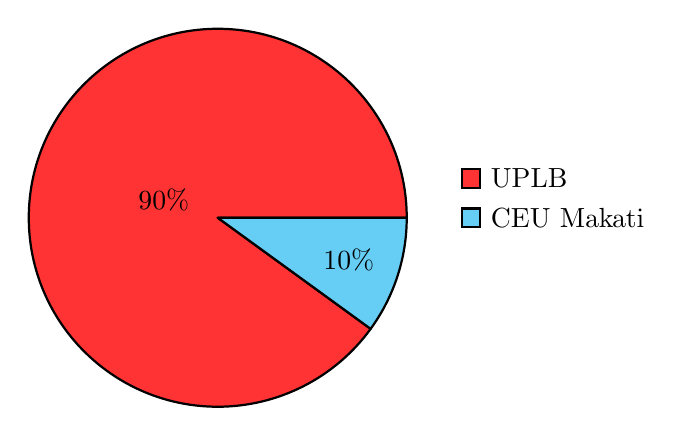
\begin{tikzpicture}[scale=0.8]
    \pie[text=legend, color={red!80, cyan!60}, radius=3]{
      90/UPLB, 
      10/CEU Makati
    }
  \end{tikzpicture}
  \caption{University Distribution of Participants}\label{fig:university}
  \Description{A pie chart showing the distribution of participants by university. 90\% of participants are from the University of the Philippines Los Baños (UPLB), represented by the red segment, while 10\% are from Centro Escolar University (CEU) Makati, represented by the cyan segment.}
\end{figure}


\begin{figure}[h]
  \centering
  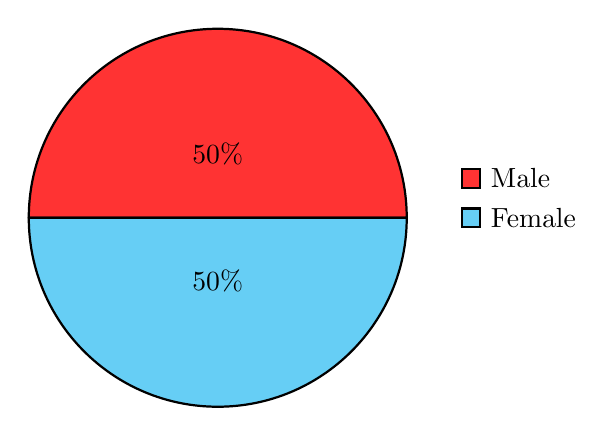
\begin{tikzpicture}[scale=0.8]
    \pie[text=legend, color={red!80, cyan!60}, radius=3]{
      50/Male,
      50/Female
    }
  \end{tikzpicture}
  \caption{Sex Distribution of Participants}\label{fig:sex}
  \Description{A pie chart showing the equal distribution of participants by sex. 50\% of participants identify as male, represented by the red segment, and 50\% identify as female, represented by the cyan segment, demonstrating perfect gender balance in the study.}
\end{figure}

In terms of academic background, there was significant disciplinary diversity, though Computer Science students constituted the largest group at 40\% (Fig.~\ref{fig:degree}). This was followed by Agricultural and Biosystems Engineering students (20\%), with the remaining 40\% equally distributed among Veterinary Medicine, Nutrition, Food Science and Technology, and Dental Medicine programs. This multidisciplinary representation strengthens the applicability of findings across different academic contexts, while still acknowledging the technical perspective that comes from the CS-heavy sample.

\begin{figure}[h]
  \centering
  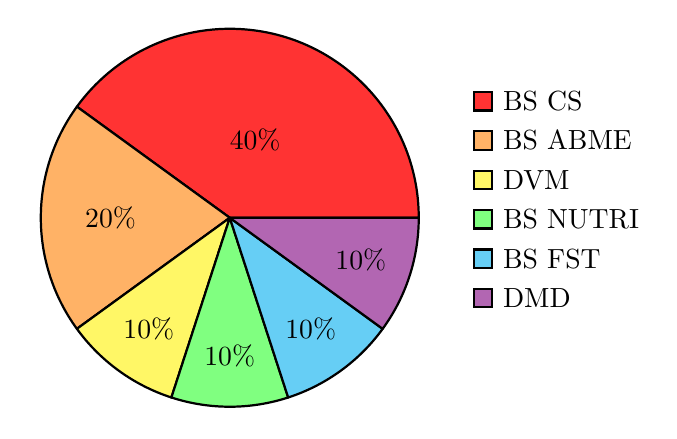
\begin{tikzpicture}[scale=0.8]
    \pie[text=legend, color={red!80, orange!60, yellow!60, green!50, cyan!60, violet!60}, radius=3]{
      40/BS CS,
      20/BS ABME,
      10/DVM,
      10/BS NUTRI,
      10/BS FST,
      10/DMD
    }
  \end{tikzpicture}
  \caption{Degree Program Distribution of Participants} \label{fig:degree}
  \Description{A pie chart showing the distribution of participants by degree program. 40\% are Bachelor of Science in Computer Science (BS CS) students, represented by the red segment; 20\% are Bachelor of Science in Agricultural and Biosystems Engineering (BS ABME) students, represented by the orange segment; 10\% are Doctor of Veterinary Medicine (DVM) students, represented by the yellow segment; 10\% are Bachelor of Science in Nutrition (BS NUTRI) students, represented by the green segment; 10\% are Bachelor of Science in Food Science and Technology (BS FST) students, represented by the cyan segment; and 10\% are Doctor of Dental Medicine (DMD) students, represented by the violet segment.}
\end{figure}

Regarding academic progression, the participants were predominantly upper-level undergraduates, with juniors (40\%) and sophomores (30\%) making up 70\% of the sample (Fig.~\ref{fig:standing}). Seniors constituted 20\%, while freshmen were the least represented at 10\%. This distribution suggests that the evaluation of STELLA comes primarily from students with moderate to significant university experience, who may have developed more established study habits and encountered various assessment methods during their academic careers.

\begin{figure}[h]
  \centering
  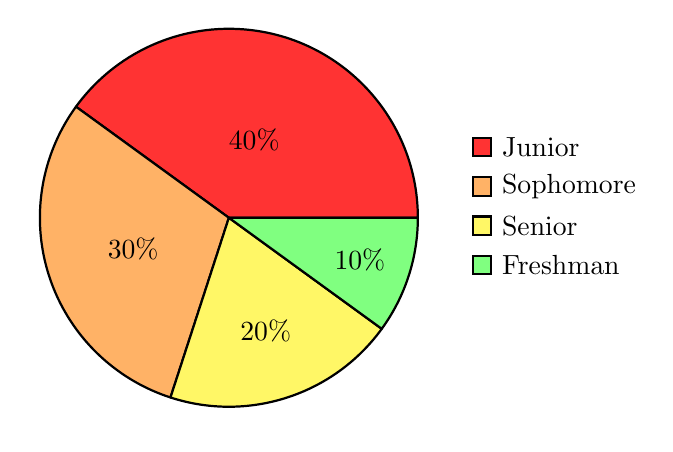
\begin{tikzpicture}[scale=0.8]
    \pie[text=legend, color={red!80, orange!60, yellow!60, green!50}, radius=3]{
      40/Junior,
      30/Sophomore,
      20/Senior,
      10/Freshman
    }
  \end{tikzpicture}
  \caption{University Standing Distribution of Participants}
  \label{fig:standing}
  \Description{A pie chart showing the distribution of participants by university standing or year level. 40\% are juniors (third-year students), represented by the red segment; 30\% are sophomores (second-year students), represented by the orange segment; 20\% are seniors (fourth-year or higher students), represented by the yellow segment; and 10\% are freshmen (first-year students), represented by the green segment.}
\end{figure}

\subsection{Statistical Analysis}
For each of the six constructs, the Wilcoxon Signed-Rank Test was
conducted to compare the satisfaction scores between STELLA and Google Classroom. The results are summarized in Table~\ref{tab:results}.

\begin{table}
  \caption{Wilcoxon Signed-Rank Test Results for STELLA vs. Google Classroom with AI Chatbot}\label{tab:results}
  \begin{tabular}{lcccc}
    \toprule
    Construct & $W_s$ & $p$-value & Result \\
    \midrule
    PE & 7.00 & 0.136 & Reject $H_{0PE}$ \\
    EE & 1.00 & 0.101 & Reject $H_{0EE}$ \\
    FC & 11.00 & 0.096 & Fail to Reject $H_{0FC}$ \\
    EC & 8.00 & 0.176 & Reject $H_{0EC}$ \\
    SA & 10.00 & 0.077 & Reject $H_{0SA}$ \\
    BI & 20.00 & 0.406 & Fail to Reject $H_{0BI}$ \\
    \bottomrule
  \end{tabular}
\end{table}

\begin{table}
  \caption{Descriptive Statistics for STELLA vs. Google Classroom with AI Chatbot by Construct}\label{tab:stats}
  \begin{tabular}{lcccc}
    \toprule
    \textbf{System and Construct} & \textbf{Mean} & \textbf{Median} & \textbf{SD} & \textbf{SE} \\
    \midrule
    Google Classroom + AI's PE & 5.76 & 6.30 & 1.490 & 0.471 \\
    STELLA's PE & 6.04 & 6.60 & 1.356 & 0.429 \\
    \midrule
    Google Classroom + AI's EE & 6.30 & 7.00 & 1.222 & 0.386 \\
    STELLA's EE & 6.57 & 7.00 & 0.994 & 0.314 \\
    \midrule
    Google Classroom + AI's FC & 6.03 & 6.25 & 0.803 & 0.254 \\
    STELLA's FC & 6.47 & 7.00 & 0.740 & 0.234 \\
    \midrule
    Google Classroom + AI's EC & 5.73 & 5.83 & 0.900 & 0.285 \\
    STELLA's EC & 6.13 & 6.67 & 1.525 & 0.482 \\
    \midrule
    Google Classroom + AI's SA & 5.55 & 5.75 & 1.428 & 0.452 \\
    STELLA's SA & 6.05 & 6.63 & 1.246 & 0.394 \\
    \midrule
    Google Classroom + AI's BI & 5.00 & 5.50 & 1.618 & 0.512 \\
    STELLA's BI & 5.23 & 5.50 & 1.757 & 0.556 \\
    \bottomrule
  \end{tabular}
\end{table}

The analysis revealed statistically significant differences across all six constructs, with STELLA consistently receiving higher ratings than Google Classroom with an AI chatbot, particularly in PE, EE, EC, and SA\@. Additionally, a thematic analysis of open-ended survey responses also identified several key areas where STELLA demonstrates advantages over the use of Google Classroom integrated with an external AI chatbot. These themes were also analyzed in the context of all 6 UTAUT+ECM factors. Hence, for each construct, the following observations were noted:


\subsubsection{Performance Expectancy}
STELLA (Mdn = 4.60) was rated significantly higher than Google Classroom $(Mdn = 3.25)$, W = 7.00, p = 0.136, indicating users perceived STELLA as substantially more effective at improving productivity and learning outcomes. This is further supported by the feedback given by the participants, as STELLA is perceived to enhance productivity and learning effectiveness without compromising academic integrity. Students appreciated that it guides rather than spoon-feeds:
\begin{itemize}
  \item \textit{“Yes, because STELLA doesn\'t automatically give answers, it simply guides you to focus on key areas\ldots this makes the process more ethical and productive.”}
  \item \textit{“It still requires me to do the assignment and not entirely rely on AI.”}
\end{itemize}
In contrast, while Google Classroom with AI chatbots may boost productivity, several respondents expressed concern that over-reliance can lead to complacency, undermining learning:
\begin{itemize}
\item \textit{“I\'ve noticed that I\'ve started to rely on [AI chatbots] more out of need than support… it raises questions about whether my learning remains authentic.”}
\end{itemize}

\subsubsection{Effort Expectancy}
STELLA's ease of use and intuitive interface was repeatedly highlighted:
\begin{itemize}
\item \textit{“The cleanness of the User Interface and the smoothness of it\ldots it\'s very good in terms of UX.”}
\end{itemize}
However, some users suggested enhancements for ease of input, such as:
\begin{itemize}
\item \textit{“Make sure [STELLA] allows typing shift+enter for a newline.”}
\end{itemize}
Conversely, Google Classroom's reliance on third-party AI chatbots created workflow fragmentation, with students needing to toggle between platforms or adjust to different chatbot behaviors.

\subsubsection{Facilitating Conditions}
Students generally felt that STELLA provided sufficient support through its prompts and feedback mechanisms:
\begin{itemize}
  \item \textit{“No concerns… it offers for me to also think critically by providing follow-up questions that may help me.”}
\end{itemize}
Suggestions for improvement mostly revolved around document compatibility and multimedia support:
\begin{itemize}
  \item \textit{“It would be helpful if it can accept various types of documents.”}
  \item \textit{“Uploading pictures.”}
\end{itemize}
For Google Classroom + AI chatbots, users pointed to a lack of integration as a key barrier:
\begin{itemize}
  \item \textit{“One improvement could be better integration between Google Classroom and the AI chatbot, allowing the bot to access assignments and deadlines directly.”}
\end{itemize}

\subsubsection{Expectation Confirmation}
Most users confirmed that STELLA met or exceeded expectations in promoting ethical and transparent learning:
\begin{itemize}
  \item \textit{“In the long run, I think it will help me more in terms of being more ethical and transparent.”}
\end{itemize}
Some did mention limitations in features like restricted summarization, especially given that STELLA was designed to not summarize text verbatim:
\begin{itemize}
  \item \textit{“The lack of the summarizing feature hinders productivity a lot for me.”}
\end{itemize}
In contrast, Google Classroom + chatbot often failed to meet expectations due to accuracy concerns and fear of being flagged for AI use:
\begin{itemize}
  \item \textit{“I am afraid that professors will think that the output I submitted is purely AI and give me a low grade for it."}
\end{itemize}

\subsubsection{Satisfaction}
Students expressed high levels of contentment with STELLA, especially with its design philosophy and ethical grounding:
\begin{itemize}
  \item \textit{“It is a safer approach to genuine understanding.”}
  \item \textit{“Nothing to improve, it\'s good.”}
\end{itemize}
Users of Google Classroom with AI chatbots reported mixed satisfaction, with many pointing out risks of plagiarism, inaccuracy, and shallow learning.

\subsubsection{Behavioral Intent}
Most STELLA users expressed a strong intent to continue using it, citing its balance of assistance and independence:
\begin{itemize}
  \item \textit{“Yes, it encourages critical thinking.”}
\end{itemize}
Some preferred traditional learning or their own methods, though they still acknowledged STELLA\'s UX strengths.

Meanwhile, Google Classroom users were more split. Some planned to continue using AI tools but expressed the need to redefine their approach to avoid over-reliance:
\begin{itemize}
  \item \textit{"I think I need to shift the way I use AI\ldots focus more on developing my own ideas before turning to AI for support."}
\end{itemize}

\section{Discussion}
\subsection{Design Implications}
One important insight gained from the design process of STELLA is that successful educational tools must be both functional and purposeful. It is not enough to simply create a working system—it must directly contribute to learning goals and values, such as promoting ethical AI use and fostering transparency. The initial plan aimed to design a learning management system that integrates an AI chatbot to support these objectives, and while several features remained static in the prototype phase, the core component—the functional workspace with a chatbot—was successfully implemented. This proved valuable in early testing and demonstrated the potential of integrating AI tools into learning environments. However, using multiple platforms in the prototype process introduced complexity, which could affect user experience by creating inconsistencies or increasing the cognitive load.

This fragmentation may have impacted users\' perception of the system\'s intuitiveness and overall reliability. Nevertheless, modular development allowed for targeted testing of specific components. The findings, especially the comparison with Google Classroom, showed that while STELLA had promising features, it fell short in Facilitating Conditions and Behavioral Intention. These results suggest that future designs, including STELLA's own future versions, must focus on improving technical accessibility and user motivation to continue using the platform. Overall, STELLA\'s core innovation—the chatbot-integrated workspace—proved appropriate and relevant, but enhancements in usability, integration, and onboarding processes are needed to realize its full potential.

\subsection{Limitations}
STELLA's current limitations stem primarily from its prototype status and the partial implementation of its features. While the chatbot-integrated workspace was functional, other elements of the LMS were static or not fully realized, limiting the scope of user testing and real-world application. This partial deployment affected the system’s overall utility, as users could not experience the full range of tools or features as intended. Additionally, STELLA lacked a structured feedback system, which is critical for monitoring user performance, offering personalized guidance, and fostering a more responsive learning environment. Without a consistent feedback loop, both learners and developers miss opportunities for reflection, improvement, and growth. These limitations, while expected in a prototype, highlight the areas that must be prioritized in future development phases to enhance functionality and user satisfaction.

\subsection{Future Work}
Future iterations of STELLA should aim to provide a more detailed mapping between its features and those of traditional learning management systems like Google Classroom. This would allow for more precise evaluations when using theoretical frameworks such as UTAUT and ECM, particularly in experimental study designs. It is also essential to further investigate the impact of the chatbot's conversational structure and responsiveness on user experience and satisfaction. Given the central role the chatbot plays in STELLA, understanding how tone, phrasing, and context-awareness affect learning behavior can guide improvements in its design. Expanding the user base for testing and simulating real educational scenarios will also be critical in validating STELLA\'s effectiveness and scalability. With these enhancements, future versions of STELLA can more confidently position themselves as robust, ethical, and transparent tools for AI-enhanced learning.

\section{Conclusion}
This paper presents STELLA as an educational platform that effectively integrates AI capabilities directly into the learning environment. When compared to the alternative approach of using Google Classroom with separate AI chatbots, STELLA demonstrated superior performance across all six evaluation metrics.

The study found STELLA's integrated approach provides substantial benefits by embedding AI assistance within the learning platform rather than requiring external tools. This design creates a transparent environment that acknowledges AI use while maintaining academic oversight, offering a practical solution to the growing presence of AI in education.

Despite being in the prototype stage with some functional limitations, STELLA's core design principles—transparent AI usage, integrated feedback systems—were validated by positive user response. The findings suggest educational institutions should embrace AI technologies by creating structured environments that guide responsible use rather than attempting to restrict access.

The research recommends future development focus on enhancing the feedback mechanisms between students, AI systems, and instructors while promoting critical thinking and genuine learning. Through such integrated approaches, educational institutions can transform AI-related challenges into opportunities for more effective and pedagogically sound learning experiences.


% \section{Template Overview}
% As noted in the introduction, the ``\verb|acmart|'' document class can
% be used to prepare many different kinds of documentation --- a
% double-anonymous initial submission of a full-length technical paper, a
% two-page SIGGRAPH Emerging Technologies abstract, a ``camera-ready''
% journal article, a SIGCHI Extended Abstract, and more --- all by
% selecting the appropriate {\itshape template style} and {\itshape
%   template parameters}.

% This document will explain the major features of the document
% class. For further information, the {\itshape \LaTeX\ User's Guide} is available from
% \url{https://www.acm.org/publications/proceedings-template}.

% \subsection{Template Styles}

% The primary parameter given to the ``\verb|acmart|'' document class is
% the {\itshape template style} which corresponds to the kind of publication
% or SIG publishing the work. This parameter is enclosed in square
% brackets and is a part of the {\verb|documentclass|} command:
% \begin{verbatim}
%   \documentclass[STYLE]{acmart}
% \end{verbatim}

% Journals use one of three template styles. All but three ACM journals
% use the {\verb|acmsmall|} template style:
% \begin{itemize}
% \item {\texttt{acmsmall}}: The default journal template style.
% \item {\texttt{acmlarge}}: Used by JOCCH and TAP.
% \item {\texttt{acmtog}}: Used by TOG.
% \end{itemize}

% The majority of conference proceedings documentation will use the {\verb|acmconf|} template style.
% \begin{itemize}
% \item {\texttt{sigconf}}: The default proceedings template style.
% \item{\texttt{sigchi}}: Used for SIGCHI conference articles.
% \item{\texttt{sigplan}}: Used for SIGPLAN conference articles.
% \end{itemize}

% \subsection{Template Parameters}

% In addition to specifying the {\itshape template style} to be used in
% formatting your work, there are a number of {\itshape template parameters}
% which modify some part of the applied template style. A complete list
% of these parameters can be found in the {\itshape \LaTeX\ User's Guide.}

% Frequently-used parameters, or combinations of parameters, include:
% \begin{itemize}
% \item {\texttt{anonymous,review}}: Suitable for a ``double-anonymous''
%   conference submission. Anonymizes the work and includes line
%   numbers. Use with the \texttt{\string\acmSubmissionID} command to print the
%   submission's unique ID on each page of the work.
% \item{\texttt{authorversion}}: Produces a version of the work suitable
%   for posting by the author.
% \item{\texttt{screen}}: Produces colored hyperlinks.
% \end{itemize}

% This document uses the following string as the first command in the
% source file:
% \begin{verbatim}
% \end{verbatim}

% \section{Modifications}

% Modifying the template --- including but not limited to: adjusting
% margins, typeface sizes, line spacing, paragraph and list definitions,
% and the use of the \verb|\vspace| command to manually adjust the
% vertical spacing between elements of your work --- is not allowed.

% {\bfseries Your document will be returned to you for revision if
%   modifications are discovered.}

% \section{Typefaces}

% The ``\verb|acmart|'' document class requires the use of the
% ``Libertine'' typeface family. Your \TeX\ installation should include
% this set of packages. Please do not substitute other typefaces. The
% ``\verb|lmodern|'' and ``\verb|ltimes|'' packages should not be used,
% as they will override the built-in typeface families.

% \section{Title Information}

% The title of your work should use capital letters appropriately -
% \url{https://capitalizemytitle.com/} has useful rules for
% capitalization. Use the {\verb|title|} command to define the title of
% your work. If your work has a subtitle, define it with the
% {\verb|subtitle|} command.  Do not insert line breaks in your title.

% If your title is lengthy, you must define a short version to be used
% in the page headers, to prevent overlapping text. The \verb|title|
% command has a ``short title'' parameter:
% \begin{verbatim}
%   \title[short title]{full title}
% \end{verbatim}

% \section{Authors and Affiliations}

% Each author must be defined separately for accurate metadata
% identification.  As an exception, multiple authors may share one
% affiliation. Authors' names should not be abbreviated; use full first
% names wherever possible. Include authors' e-mail addresses whenever
% possible.

% Grouping authors' names or e-mail addresses, or providing an ``e-mail
% alias,'' as shown below, is not acceptable:
% \begin{verbatim}
%   \author{Brooke Aster, David Mehldau}
%   \email{dave,judy,steve@university.edu}
%   \email{firstname.lastname@phillips.org}
% \end{verbatim}

% The \verb|authornote| and \verb|authornotemark| commands allow a note
% to apply to multiple authors --- for example, if the first two authors
% of an article contributed equally to the work.

% If your author list is lengthy, you must define a shortened version of
% the list of authors to be used in the page headers, to prevent
% overlapping text. The following command should be placed just after
% the last \verb|\author{}| definition:
% \begin{verbatim}
%   \renewcommand{\shortauthors}{McCartney, et al.}
% \end{verbatim}
% Omitting this command will force the use of a concatenated list of all
% of the authors' names, which may result in overlapping text in the
% page headers.

% The article template's documentation, available at
% \url{https://www.acm.org/publications/proceedings-template}, has a
% complete explanation of these commands and tips for their effective
% use.

% Note that authors' addresses are mandatory for journal articles.

% \section{Rights Information}

% Authors of any work published by ACM will need to complete a rights
% form. Depending on the kind of work, and the rights management choice
% made by the author, this may be copyright transfer, permission,
% license, or an OA (open access) agreement.

% Regardless of the rights management choice, the author will receive a
% copy of the completed rights form once it has been submitted. This
% form contains \LaTeX\ commands that must be copied into the source
% document. When the document source is compiled, these commands and
% their parameters add formatted text to several areas of the final
% document:
% \begin{itemize}
% \item the ``ACM Reference Format'' text on the first page.
% \item the ``rights management'' text on the first page.
% \item the conference information in the page header(s).
% \end{itemize}

% Rights information is unique to the work; if you are preparing several
% works for an event, make sure to use the correct set of commands with
% each of the works.

% The ACM Reference Format text is required for all articles over one
% page in length, and is optional for one-page articles (abstracts).

% \section{CCS Concepts and User-Defined Keywords}

% Two elements of the ``acmart'' document class provide powerful
% taxonomic tools for you to help readers find your work in an online
% search.

% The ACM Computing Classification System ---
% \url{https://www.acm.org/publications/class-2012} --- is a set of
% classifiers and concepts that describe the computing
% discipline. Authors can select entries from this classification
% system, via \url{https://dl.acm.org/ccs/ccs.cfm}, and generate the
% commands to be included in the \LaTeX\ source.

% User-defined keywords are a comma-separated list of words and phrases
% of the authors' choosing, providing a more flexible way of describing
% the research being presented.

% CCS concepts and user-defined keywords are required for for all
% articles over two pages in length, and are optional for one- and
% two-page articles (or abstracts).

% \section{Sectioning Commands}

% Your work should use standard \LaTeX\ sectioning commands:
% \verb|\section|, \verb|\subsection|, \verb|\subsubsection|,
% \verb|\paragraph|, and \verb|\subparagraph|. The sectioning levels up to
% \verb|\subsusection| should be numbered; do not remove the numbering
% from the commands.

% Simulating a sectioning command by setting the first word or words of
% a paragraph in boldface or italicized text is {\bfseries not allowed.}

% Below are examples of sectioning commands.

% \subsection{Subsection}
% \label{sec:subsection}

% This is a subsection.

% \subsubsection{Subsubsection}
% \label{sec:subsubsection}

% This is a subsubsection.

% \paragraph{Paragraph}

% This is a paragraph.

% \subparagraph{Subparagraph}

% This is a subparagraph.

% \section{Tables}

% The ``\verb|acmart|'' document class includes the ``\verb|booktabs|''
% package --- \url{https://ctan.org/pkg/booktabs} --- for preparing
% high-quality tables.

% Table captions are placed {\itshape above} the table.

% Because tables cannot be split across pages, the best placement for
% them is typically the top of the page nearest their initial cite.  To
% ensure this proper ``floating'' placement of tables, use the
% environment \textbf{table} to enclose the table's contents and the
% table caption.  The contents of the table itself must go in the
% \textbf{tabular} environment, to be aligned properly in rows and
% columns, with the desired horizontal and vertical rules.  Again,
% detailed instructions on \textbf{tabular} material are found in the
% \textit{\LaTeX\ User's Guide}.

% Immediately following this sentence is the point at which
% Table~\ref{tab:freq} is included in the input file; compare the
% placement of the table here with the table in the printed output of
% this document.

% \begin{table}
%   \caption{Frequency of Special Characters}
%   \label{tab:freq}
%   \begin{tabular}{ccl}
%     \toprule
%     Non-English or Math&Frequency&Comments\\
%     \midrule
%     \O & 1 in 1,000& For Swedish names\\
%     $\pi$ & 1 in 5& Common in math\\
%     \$ & 4 in 5 & Used in business\\
%     $\Psi^2_1$ & 1 in 40,000& Unexplained usage\\
%   \bottomrule
% \end{tabular}
% \end{table}

% To set a wider table, which takes up the whole width of the page's
% live area, use the environment \textbf{table*} to enclose the table's
% contents and the table caption.  As with a single-column table, this
% wide table will ``float'' to a location deemed more
% desirable. Immediately following this sentence is the point at which
% Table~\ref{tab:commands} is included in the input file; again, it is
% instructive to compare the placement of the table here with the table
% in the printed output of this document.

% \begin{table*}
%   \caption{Some Typical Commands}
%   \label{tab:commands}
%   \begin{tabular}{ccl}
%     \toprule
%     Command &A Number & Comments\\
%     \midrule
%     \texttt{{\char'134}author} & 100& Author \\
%     \texttt{{\char'134}table}& 300 & For tables\\
%     \texttt{{\char'134}table*}& 400& For wider tables\\
%     \bottomrule
%   \end{tabular}
% \end{table*}

% Always use midrule to separate table header rows from data rows, and
% use it only for this purpose. This enables assistive technologies to
% recognise table headers and support their users in navigating tables
% more easily.

% \section{Math Equations}
% You may want to display math equations in three distinct styles:
% inline, numbered or non-numbered display.  Each of the three are
% discussed in the next sections.

% \subsection{Inline (In-text) Equations}
% A formula that appears in the running text is called an inline or
% in-text formula.  It is produced by the \textbf{math} environment,
% which can be invoked with the usual
% \texttt{{\char'134}begin\,\ldots{\char'134}end} construction or with
% the short form \texttt{\$\,\ldots\$}. You can use any of the symbols
% and structures, from $\alpha$ to $\omega$, available in
% % \LaTeX~\cite{Lamport:LaTeX}; this section will simply show a few
% examples of in-text equations in context. Notice how this equation:
% \begin{math}
%   \lim_{n\rightarrow \infty}x=0
% \end{math},
% set here in in-line math style, looks slightly different when
% set in display style.  (See next section).

% \subsection{Display Equations}
% A numbered display equation---one set off by vertical space from the
% text and centered horizontally---is produced by the \textbf{equation}
% environment. An unnumbered display equation is produced by the
% \textbf{displaymath} environment.

% Again, in either environment, you can use any of the symbols and
% structures available in \LaTeX\@; this section will just give a couple
% of examples of display equations in context.  First, consider the
% equation, shown as an inline equation above:
% \begin{equation}
%   \lim_{n\rightarrow \infty}x=0
% \end{equation}
% Notice how it is formatted somewhat differently in
% the \textbf{displaymath}
% environment.  Now, we'll enter an unnumbered equation:
% \begin{displaymath}
%   \sum_{i=0}^{\infty} x + 1
% \end{displaymath}
% and follow it with another numbered equation:
% \begin{equation}
%   \sum_{i=0}^{\infty}x_i=\int_{0}^{\pi+2} f
% \end{equation}
% just to demonstrate \LaTeX's able handling of numbering.

% \section{Figures}

% The ``\verb|figure|'' environment should be used for figures. One or
% more images can be placed within a figure. If your figure contains
% third-party material, you must clearly identify it as such, as shown
% in the example below.
% \begin{figure}[h]
%   \centering
%   \includegraphics[width=\linewidth]{sample-franklin}
%   \caption{1907 Franklin Model D roadster. Photograph by Harris \&
%     Ewing, Inc. [Public domain], via Wikimedia
%     Commons. (\url{https://goo.gl/VLCRBB}).}
%   \Description{A woman and a girl in white dresses sit in an open car.}
% \end{figure}

% Your figures should contain a caption which describes the figure to
% the reader.

% Figure captions are placed {\itshape below} the figure.

% Every figure should also have a figure description unless it is purely
% decorative. These descriptions convey what’s in the image to someone
% who cannot see it. They are also used by search engine crawlers for
% indexing images, and when images cannot be loaded.

% A figure description must be unformatted plain text less than 2000
% characters long (including spaces).  {\bfseries Figure descriptions
%   should not repeat the figure caption – their purpose is to capture
%   important information that is not already provided in the caption or
%   the main text of the paper.} For figures that convey important and
% complex new information, a short text description may not be
% adequate. More complex alternative descriptions can be placed in an
% appendix and referenced in a short figure description. For example,
% provide a data table capturing the information in a bar chart, or a
% structured list representing a graph.  For additional information
% regarding how best to write figure descriptions and why doing this is
% so important, please see
% \url{https://www.acm.org/publications/taps/describing-figures/}.

% \subsection{The ``Teaser Figure''}

% A ``teaser figure'' is an image, or set of images in one figure, that
% are placed after all author and affiliation information, and before
% the body of the article, spanning the page. If you wish to have such a
% figure in your article, place the command immediately before the
% \verb|\maketitle| command:
% \begin{verbatim}
%   \begin{teaserfigure}
%     \includegraphics[width=\textwidth]{sampleteaser}
%     \caption{figure caption}
%     \Description{figure description}
%   \end{teaserfigure}
% \end{verbatim}

% \section{Citations and Bibliographies}

% The use of \BibTeX\ for the preparation and formatting of one's
% references is strongly recommended. Authors' names should be complete
% --- use full first names (``Donald E. Knuth'') not initials
% (``D. E. Knuth'') --- and the salient identifying features of a
% reference should be included: title, year, volume, number, pages,
% article DOI, etc.


% Using the BibLaTeX system, the bibliography is included in your source
% document with the following command, placed just before the \verb|\end{document}| command:
% \begin{verbatim}
%   \printbibliography
% \end{verbatim}

% The command \verb|\addbibresource{bibfile}| declares the \BibTeX\ file to use
% in the {\bfseries preamble} (before the command
% ``\verb|\begin{document}|'') of your \LaTeX\ source
% where ``\verb|bibfile|'' is the name, \emph{with} the ``\verb|.bib|'' suffix.
% Notice that \verb|\addbibresource| takes only one argument: to declare multiple files,
% use multiple instances of the command.

% Citations and references are numbered by default. A small number of
% ACM publications have citations and references formatted in the
% ``author year'' style; for these exceptions, please pass the option \verb|style=acmauthoryear|
% to the \verb|biblatex| package loaded in the {\bfseries preamble} (before the command
% ``\verb|\begin{document}|'') of your \LaTeX\ source.


  % Some examples.  A paginated journal article \cite{Abril07}, an
  % enumerated journal article \cite{Cohen07}, a reference to an entire
  % issue \cite{JCohen96}, a monograph (whole book) \cite{Kosiur01}, a
  % monograph/whole book in a series (see 2a in spec. document)
  % \cite{Harel79}, a divisible-book such as an anthology or compilation
  % \cite{Editor00} followed by the same example, however we only output
  % the series if the volume number is given \cite{Editor00a} (so
  % Editor00a's series should NOT be present since it has no vol. no.),
  % a chapter in a divisible book \cite{Spector90}, a chapter in a
  % divisible book in a series \cite{Douglass98}, a multi-volume work as
  % book \cite{Knuth97}, a couple of articles in a proceedings (of a
  % conference, symposium, workshop for example) (paginated proceedings
  % article) \cite{Andler79, Hagerup1993}, a proceedings article with
  % all possible elements \cite{Smith10}, an example of an enumerated
  % proceedings article \cite{VanGundy07}, an informally published work
  % \cite{Harel78}, a couple of preprints \cite{Bornmann2019,
  %   AnzarootPBM14}, a doctoral dissertation \cite{Clarkson85}, a
  % master's thesis: \cite{anisi03}, an online document / world wide web
  % resource \cite{Thornburg01, Ablamowicz07, Poker06}, a video game
  % (Case 1) \cite{Obama08} and (Case 2) \cite{Novak03} and \cite{Lee05}
  % and (Case 3) a patent \cite{JoeScientist001}, work accepted for
  % publication \cite{rous08}, 'YYYYb'-test for prolific author
  % \cite{SaeediMEJ10} and \cite{SaeediJETC10}. Other cites might
  % contain 'duplicate' DOI and URLs (some SIAM articles)
  % \cite{Kirschmer:2010:AEI:1958016.1958018}. Boris / Barbara Beeton:
  % multi-volume works as books \cite{MR781536} and \cite{MR781537}. A
  % couple of citations with DOIs:
  % \cite{2004:ITE:1009386.1010128,Kirschmer:2010:AEI:1958016.1958018}. Online
  % citations: \cite{TUGInstmem, Thornburg01, CTANacmart}.
  % Data Artifacts: \cite{UMassCitations}.
  % Software project: ~\cite{cgal,delebecque:hal-02090402}. Software Version: ~\cite{gf-tag-sound-repo,}. Software Module: ~\cite{cgal:lp-gi-20a}. Code fragment: ~\cite{simplemapper}.

% \section{Acknowledgments}

% Identification of funding sources and other support, and thanks to
% individuals and groups that assisted in the research and the
% preparation of the work should be included in an acknowledgment
% section, which is placed just before the reference section in your
% document.

% This section has a special environment:
% \begin{verbatim}
%   \begin{acks}
%   ...
%   \end{acks}
% \end{verbatim}
% so that the information contained therein can be more easily collected
% during the article metadata extraction phase, and to ensure
% consistency in the spelling of the section heading.

% Authors should not prepare this section as a numbered or unnumbered {\verb|\section|}; please use the ``{\verb|acks|}'' environment.

% If your work needs an appendix, add it before the
% ``\verb|\end{document}|'' command at the conclusion of your source
% document.

% Start the appendix with the ``\verb|appendix|'' command:
% \begin{verbatim}
%   \appendix
% \end{verbatim}
% and note that in the appendix, sections are lettered, not
% numbered. This document has two appendices, demonstrating the section
% and subsection identification method.

% \section{Multi-language papers}

% Papers may be written in languages other than English or include
% titles, subtitles, keywords and abstracts in different languages (as a
% rule, a paper in a language other than English should include an
% English title and an English abstract).  Use \verb|language=...| for
% every language used in the paper.  The last language indicated is the
% main language of the paper.  For example, a French paper with
% additional titles and abstracts in English and German may start with
% the following command
% \begin{verbatim}
% \documentclass[sigconf, language=english, language=german,
%                language=french]{acmart}
% \end{verbatim}

% The title, subtitle, keywords and abstract will be typeset in the main
% language of the paper.  The commands \verb|\translatedXXX|, \verb|XXX|
% begin title, subtitle and keywords, can be used to set these elements
% in the other languages.  The environment \verb|translatedabstract| is
% used to set the translation of the abstract.  These commands and
% environment have a mandatory first argument: the language of the
% second argument.  See \verb|sample-sigconf-i13n.tex| file for examples
% of their usage.

% \section{SIGCHI Extended Abstracts}

% The ``\verb|sigchi-a|'' template style (available only in \LaTeX\ and
% not in Word) produces a landscape-orientation formatted article, with
% a wide left margin. Three environments are available for use with the
% ``\verb|sigchi-a|'' template style, and produce formatted output in
% the margin:
% \begin{description}
% \item[\texttt{sidebar}:]  Place formatted text in the margin.
% \item[\texttt{marginfigure}:] Place a figure in the margin.
% \item[\texttt{margintable}:] Place a table in the margin.
% \end{description}

% %%
% %% The acknowledgments section is defined using the "acks" environment
% %% (and NOT an unnumbered section). This ensures the proper
% %% identification of the section in the article metadata, and the
% %% consistent spelling of the heading.
% \begin{acks}
% To Robert, for the bagels and explaining CMYK and color spaces.
% \end{acks}

%%
%% Print the bibliography
%%
\bibliography{references}

%%
%% If your work has an appendix, this is the place to put it.
\appendix

% \section{Research Methods}

% \subsection{Part One}

% Lorem ipsum dolor sit amet, consectetur adipiscing elit. Morbi
% malesuada, quam in pulvinar varius, metus nunc fermentum urna, id
% sollicitudin purus odio sit amet enim. Aliquam ullamcorper eu ipsum
% vel mollis. Curabitur quis dictum nisl. Phasellus vel semper risus, et
% lacinia dolor. Integer ultricies commodo sem nec semper.

% \subsection{Part Two}

% Etiam commodo feugiat nisl pulvinar pellentesque. Etiam auctor sodales
% ligula, non varius nibh pulvinar semper. Suspendisse nec lectus non
% ipsum convallis congue hendrerit vitae sapien. Donec at laoreet
% eros. Vivamus non purus placerat, scelerisque diam eu, cursus
% ante. Etiam aliquam tortor auctor efficitur mattis.

% \section{Online Resources}

% Nam id fermentum dui. Suspendisse sagittis tortor a nulla mollis, in
% pulvinar ex pretium. Sed interdum orci quis metus euismod, et sagittis
% enim maximus. Vestibulum gravida massa ut felis suscipit
% congue. Quisque mattis elit a risus ultrices commodo venenatis eget
% dui. Etiam sagittis eleifend elementum.

% Nam interdum magna at lectus dignissim, ac dignissim lorem
% rhoncus. Maecenas eu arcu ac neque placerat aliquam. Nunc pulvinar
% massa et mattis lacinia.

\end{document}
